\documentclass[runningheads]{llncs}

\usepackage[T1]{fontenc}

\usepackage{graphicx} 

\usepackage{hyperref}
\usepackage{color}
\usepackage{booktabs}
\usepackage{subcaption}
\renewcommand\UrlFont{\color{blue}\rmfamily}

\raggedbottom

\begin{document}

\title{Monte Carlo Control and SARSA on TextFlappyBird: A Comparative Analysis}

\titlerunning{MCC and SARSA on TextFlappyBird}

\author{Jean-Vincent Martini}
\authorrunning{J.-V. Martini}

\institute{CentraleSupélec}
 
\maketitle    

\vspace*{-0.7cm}
  
\begin{abstract}
This report evaluates Monte Carlo Control and SARSA algorithms on state- and screen-based versions of the \href{https://gitlab-research.centralesupelec.fr/stergios.christodoulidis/text-flappy-bird-gym}{TextFlappyBird} environment. We analyze hyperparameter sensitivity, investigate policy transferability across configurations, and compare agent performance using rewards and scores. The report concludes with a discussion of observed trends and potential improvements. The code is available at \url{https://github.com/JeanJNMV/MDS-RL_Text_Flappy_Bird}.
\keywords{Reinforcement Learning \and Deep Learning \and Monte Carlo Control \and SARSA \and TextFlappyBird}
\end{abstract}
%
%
\vspace*{-0.7cm}

\section{Introduction and Problem Definition}

The objective of this project is to apply reinforcement learning (RL) techniques to master a simplified, terminal-based variant of the popular game Flappy Bird, known as Text Flappy Bird (TFB). In this environment, the player controls a simple unit-element character navigating through a series of pipe obstacles, aiming to maximize survival time and score. 
The problem is modeled using two distinct variations of the TFB environment, provided via a custom OpenAI Gym implementation: the simple version and the screen  version. Each version presents unique challenges in terms of observation space and complexity, requiring different approaches to policy learning and value estimation. To solve this environment, we formulate the gameplay as a Markov Decision Process and investigate two specific RL algorithms: the Monte Carlo Control method and the Sarsa($\lambda$) algorithm.
By implementing these agents, this report aims to evaluate and compare their convergence and overall performance across both environment versions. Furthermore, we conduct a sensitivity analysis on key hyperparameters and investigate the transferability of the learned policies to provide deeper insights into the behavior of both algorithms.

\section{Implementation Details}
\paragraph{Environment Setup and State Representation.} Both TFB variants share the
same dynamics: the action space consists of two actions, $0$ (Idle) and $1$ (Flap),
the agent receives a reward of $+1$ per step alive (making the reward proportional to the score since the score increases by 1 for every 10 steps) and an episode terminates on
collision. They differ only in their observation space. The simple version provides
a tuple $(dx, dy)$ representing the horizontal and vertical distances to the center
of the nearest pipe gap, restricting the state space to the most critical navigational
information. The screen version instead exposes the full $20 \times 15$ game grid as
a \texttt{gym.spaces.Box}, where each cell encodes an entity: $0$ (background),
$1$ (alive player), $2$ (pipe), or $3$ (dead player), requiring the agent to
implicitly extract geometric features from the raw spatial layout. 

\paragraph{Agents and Algorithms.} We implemented two classical RL algorithms. Both utilize an $\epsilon$-greedy exploration strategy with exponential decay. For the screen environment, two complementary state representations are used. In the hash-based variant, the raw grid array is serialized into a nested tuple usable as a dictionary key, preserving full grid information at the cost of a large, non-generalizing state space. In the tile-coding variant, a compact feature vector $(d_x, d_y)$ is extracted from the screen and encoded using $8$ overlapping tilings over a $4\times4$ grid, enabling generalization across nearby states through linear function approximation.

The Monte Carlo Control (MCC) agent learns from complete episodes. At the end of each episode, the cumulative discounted return $G_t$ is computed backwards from the terminal state. The Q-values are updated for every visited state-action pair using a constant step-size $\alpha$:
$Q(S_t, A_t) \leftarrow Q(S_t, A_t) + \alpha (G_t - Q(S_t, A_t))$. 

The Sarsa($\lambda$) agent, in contrast, utilizes eligibility traces to propagate delayed rewards back to recently visited states more efficiently\cite{sutton2018reinforcement}. Our implementation increments an accumulating trace $E(s,a)$ upon visitation. The error $\delta_t$ and subsequent Q-value updates for all active traces are defined as:
$\delta_t = R_{t+1} + \gamma Q(S_{t+1}, A_{t+1}) - Q(S_t, A_t)$ and
$Q(s, a) \leftarrow Q(s, a) + \alpha \delta_t E(s, a)$.
To optimize memory and computational performance during training, any traces that decay below a negligible threshold ($1 \times 10^{-10}$) are dynamically deleted.


\section{Evaluation and Results}
\paragraph{Performance Comparison between Monte Carlo Control and SARSA.} Agents were trained for 25\,000 episodes and evaluated over 200 episodes (fewer for tile coding due to slower inference) on the training setup (\texttt{height=15}, \texttt{width=20}, \texttt{pipe\_gap=4}), with a 50\,000-step cap per episode (max score: 4999). Figure~\ref{fig:train_scores} shows training curves and Table~\ref{tab:results} reports results. Due to a heavily skewed score distribution, the median better reflects typical performance than the mean, which is influenced by rare high scores and often too close to the standard deviation.

\begin{figure}[ht]
    \centering
    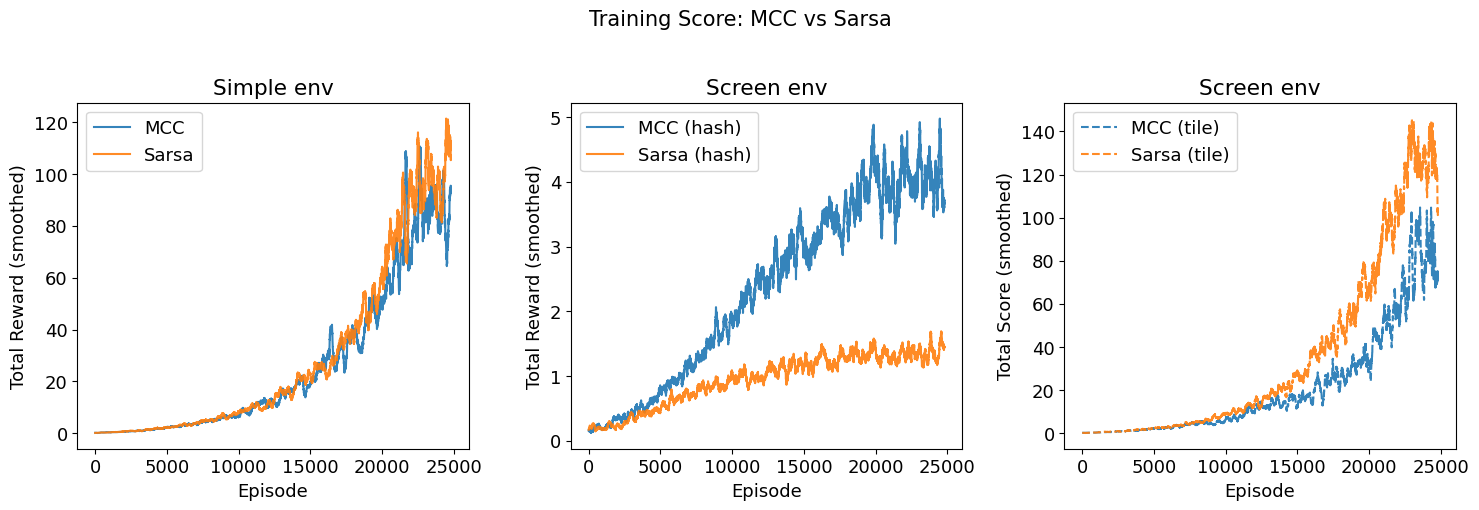
\includegraphics[width=\textwidth]{figures/train_scores.png}
    \caption{Training scores for all agents and environment configurations. The curves are smoothed using a moving average with a window size of 100 episodes for better visualization. The training configuration is $\alpha=0.01$, $\gamma=0.99$, $\lambda=0.8$ (for Sarsa), and $\epsilon$-decay$=0.9998$.}
    \label{fig:train_scores}
\end{figure}


\begin{table}[ht]
\centering
\small
\resizebox{\textwidth}{!}{
\begin{tabular}{llrrrrrr}
\hline
\textbf{Agent} & \textbf{Env} & \textbf{Mean Rew.} & \textbf{Std Rew.} & \textbf{Mean Score} & \textbf{Std Score} & \textbf{Med.\ Rew.} & \textbf{Med.\ Score} \\
\hline
MCC        & v0        & 50000.0 &    0.0 & 4999.00 &   0.00 & 50000.0 & 4999.00 \\
Sarsa      & v0        &  7489.6 & 8028.2 &  747.66 & 802.82 &  4338.0 &  432.50 \\
MCC        & screen-v0 &    53.5 &   36.8 &    4.11 &   3.67 &    43.0 &    3.00 \\
Sarsa      & screen-v0 &    22.9 &   14.5 &    1.06 &   1.47 &    19.0 &    1.00 \\
MCC Tile   & screen-v0 & 50000.0 &    0.0 & 4999.00 &   0.00 & 50000.0 & 4999.00 \\
Sarsa Tile & screen-v0 & 50000.0 &    0.0 & 4999.00 &   0.00 & 50000.0 & 4999.00 \\
\hline
\end{tabular}}
\caption{Evaluation results per agent and environment configuration. The maximum possible reward is 50\,000 (corresponding to a score of 4999) due to the step cap.}
\label{tab:results}
\end{table}

In the simple environment, both agents learned effective policies, but MCC was more stable at evaluation, consistently reaching 4999, while Sarsa remained less stable despite similar training scores. In the screen environment, tile coding proved to be essential. Both MCC and Sarsa with tile coding achieved maximal evaluation performance, whereas hash-based agents failed to generalize across the large state space, producing much lower scores. The overall gap in performance between MCC and Sarsa could stem from Sarsa's bootstrapping, where Q-updates depend on current next-state estimates, introducing variance, while MCC uses full episode returns, yielding lower-variance and more reliable estimates in this case.

Figure~\ref{fig:state_value_policy} compares learned value functions and policies. In the simple and tile-coded settings, both agents learned similar value landscapes, with high values near the screen center (pipe gap), and converged almost to the same policy: often flap below the gap, idle above. With the hash-based representation, no meaningful value function or policy could be visualized due to the large sparse state space. We can still observe that most states had zero value estimates, indicating its failure to learn a coherent strategy.

\paragraph{Hyperparameter Sensitivity Analysis.} We conducted a sensitivity analysis on key hyperparameters, including the learning rate $\alpha$, discount factor $\gamma$, and $\epsilon$-decay. We only considered the simple environment and the tile-based screen environment, as the hash-based agents did not learn meaningful policies. For each agent and environment, we performed an ablation study on its hyperparameters. The number of training episodes was reduced to 5\,000 and the number of explored values per hyperparameter was limited due to computational constraints. Figure~\ref{fig:sensitivity} in the Appendix shows the results of this analysis. Overall, both MCC agents demonstrated greater robustness to hyperparameter variations, with a wider range of values yielding good performance. In contrast, the Sarsa agent of the simple environment showed more sensitivity compared to its tile-based counterpart, which was more stable across different hyperparameter settings. However, all models showed sensitivity to the learning rate $\alpha$, highlighting the importance of careful tuning to ensure convergence and optimal performance. It is important to keep in mind that this analysis is not exhaustive due to the limited number of explored values and training episodes, and further investigation with a more comprehensive grid search or automated hyperparameter optimization could provide deeper insights into the stability and performance of these agents.

\begin{figure}[htbp]
    \centering
    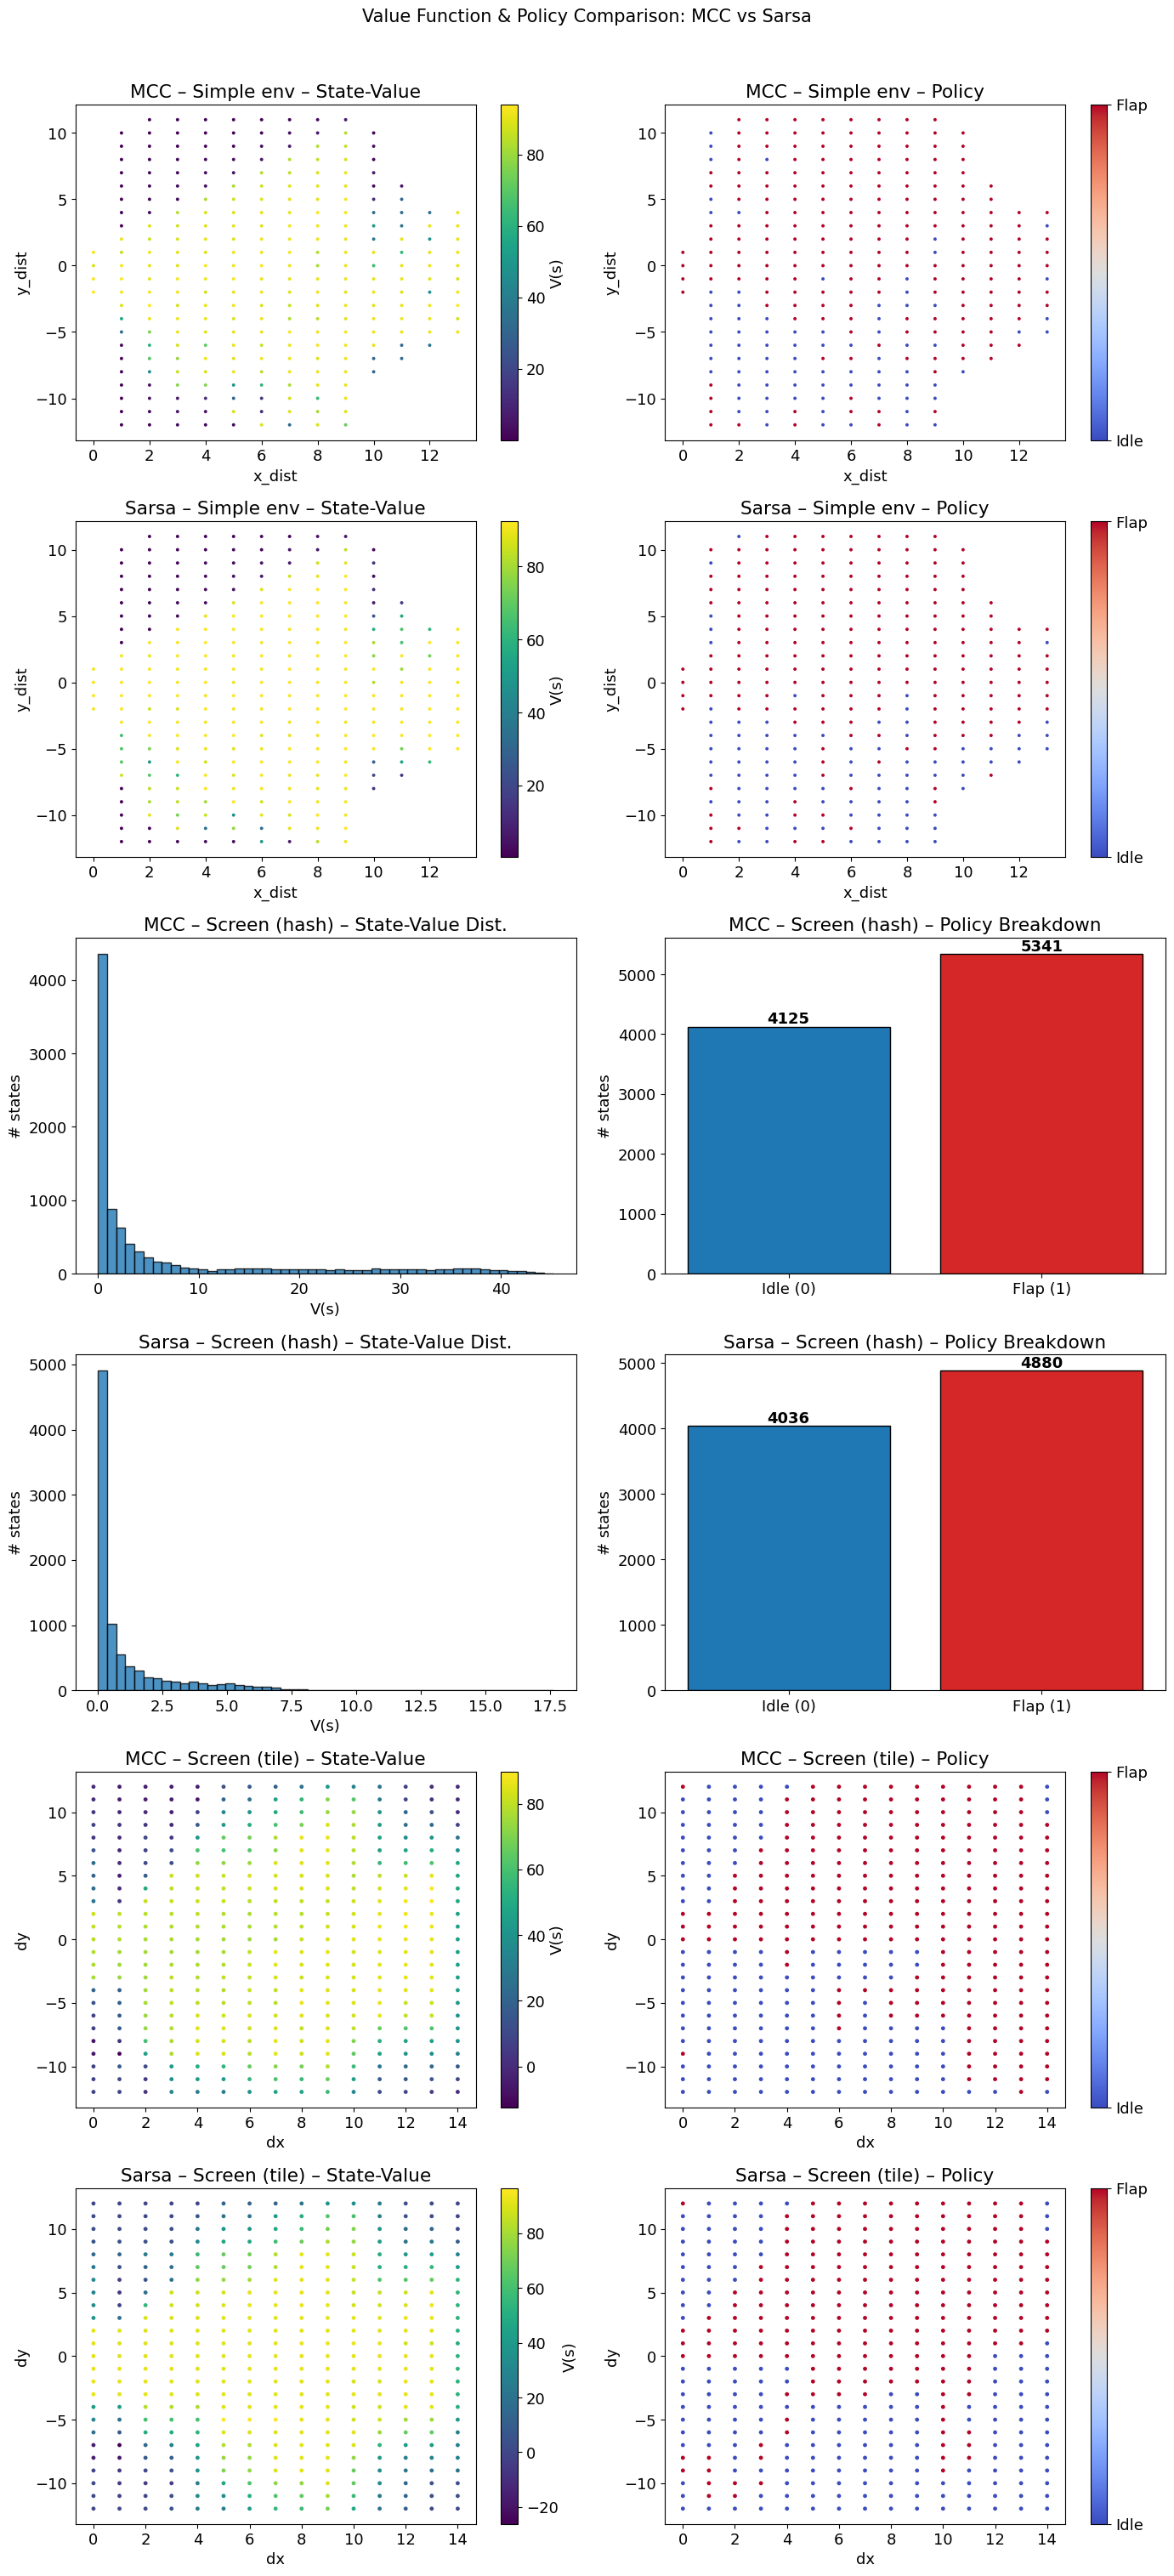
\includegraphics[width=0.7\textwidth]{figures/state_value.png}
    \caption{State-value function estimates (left) and Policy visualization (right) for all agents. For the screen environment with the hash-based representation, since the number of states is extremely large, we only visualize the repartition of value estimates across the state in the left column and the repartition between the two actions in the right column.}
    \label{fig:state_value_policy}
\end{figure}

\paragraph{Transferability of Learned Policies through Different Environment Configurations.} We evaluate the generalization of the learned policies across different environment configurations, specifically varying the screen dimensions and pipe gap. We trained the 3 variants of our best performing agent, the MCC, on the original configuration (\texttt{height=15}, \texttt{width=20}, \texttt{pipe\_gap=4}) and evaluated them on 7 new configurations, including shorter and taller screens and pipe gaps. Figure~\ref{fig:transferability} shows the results of this evaluation. Both the simple and tile-based agents showed the same degree of generalization, with strong performance for a wider pipe gap and a slightly shorter screen, but a significant drop in performance for all other configurations. This suggests that the learned policies rely heavily on the specific geometry of the training environment, and that even small changes in the layout can significantly impact performance. The hash-based agent, which already struggled to learn a good policy in the original configuration, performed poorly across all new configurations, further highlighting its lack of generalization capabilities.
 
\begin{figure}[ht]
    \centering
    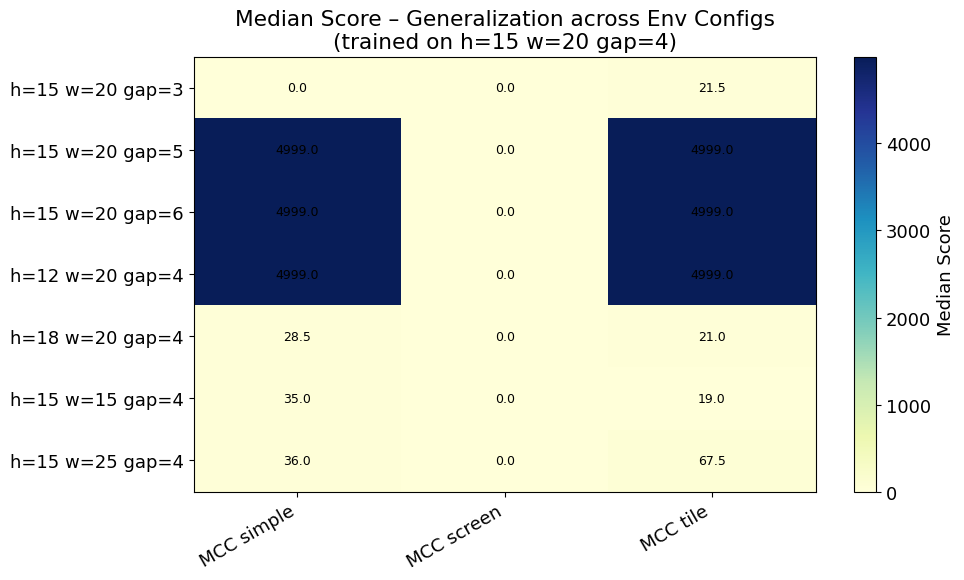
\includegraphics[width=0.9\textwidth]{figures/transferability.png}
    \caption{Generalization performance of the MCC agents across different environment configurations. Each section of the plot corresponds to a different configuration on which the agents were evaluated after being trained on the original configuration (\texttt{height=15}, \texttt{width=20}, \texttt{pipe\_gap=4}).}
    \label{fig:transferability}
\end{figure}

\paragraph{Key Limitations for the Real Flappy Bird Game.}
Although some agents perform well in TFB, transferring them to the original \href{https://github.com/Talendar/flappy-bird-gym}{Flappy Bird Gym} faces key limitations. Agents in the simple environment depend on a compact $(dx, dy)$ observation not provided by the original game, requiring feature extraction. Hash-based screen agents are highly unfit for this task, as changes in resolution or layout create unseen states and invalidate the Q-table. Tile-coding agents are more promising due to their use of $(dx, dy)$ features and robustness to small variations, but they still require careful parameter tuning and may struggle with increased complexity, noise, faster dynamics, and richer visuals. More generally, all methods rely on tabular or linear representations that do not scale well to the original game's visual complexity. Prior work on Flappy Bird includes DQN-based methods \cite{appiah2018playing,chen2015deep}, genetic algorithms \cite{gan2022flappy}, tabular Q-learning \cite{vu2020flapai}, and neuroevolution \cite{brandao2019reinforcement}.

\section{Conclusion}

This study shows that both Monte Carlo Control and Sarsa can learn effective policies in TextFlappyBird, with MCC demonstrating greater stability and reliability overall. Feature representation plays a critical role, as tile coding enables strong generalization while hash-based methods fail in high-dimensional settings. Finally, limited transferability across environment variations highlights the need for more robust function approximation methods to handle increased complexity.

% ---- Bibliography ----
{\footnotesize
\bibliographystyle{splncs04}
\bibliography{mybibliography}
}

\clearpage
\appendix

\section{Figures for Hyperparameter Sensitivity Analysis}

\begin{figure}[htbp]
\centering
 
\begin{subfigure}[b]{0.49\textwidth}
    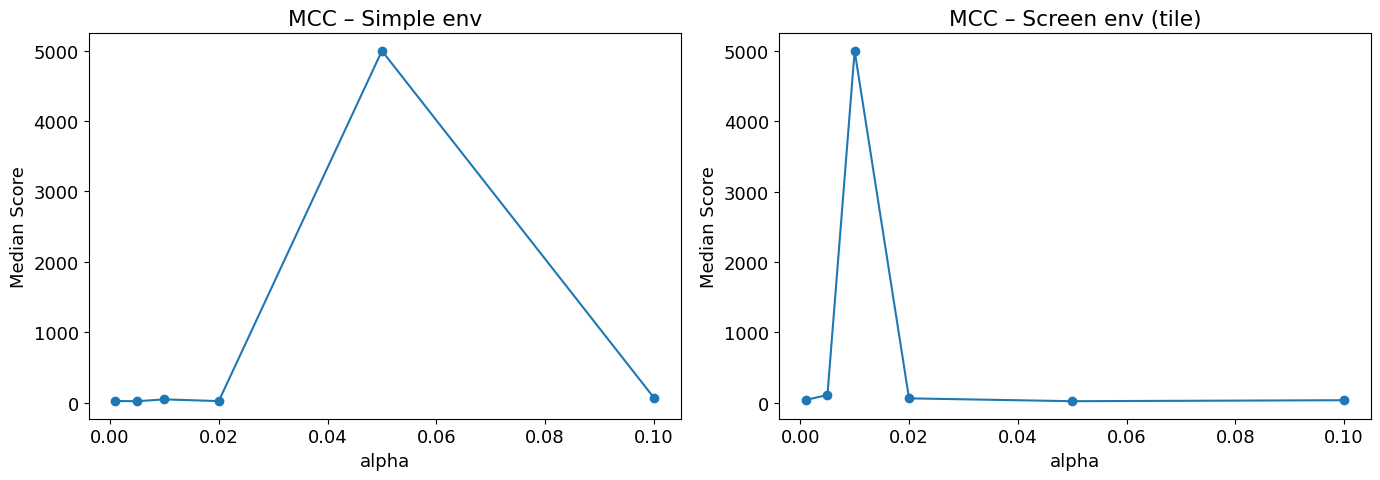
\includegraphics[width=\textwidth]{figures/MCC_alpha.png}
    \caption{MCC - Learning Rate $\alpha$}
\end{subfigure}
\hfill
\begin{subfigure}[b]{0.49\textwidth}
    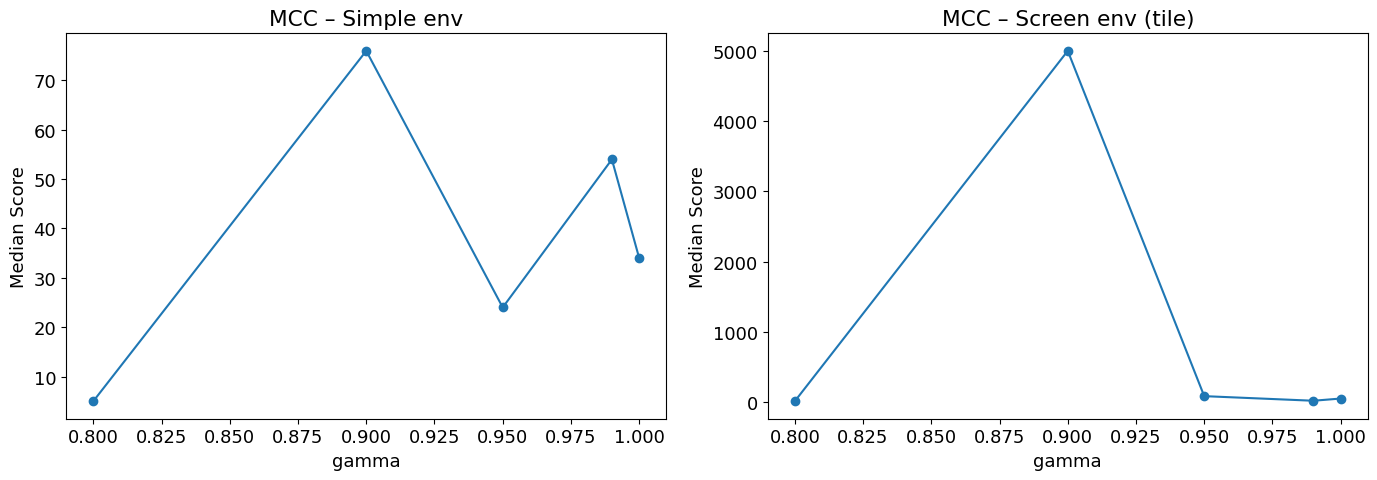
\includegraphics[width=\textwidth]{figures/MCC_gamma.png}
    \caption{MCC - Discount Factor $\gamma$}
\end{subfigure}
\hfill
\begin{subfigure}[b]{0.49\textwidth}
    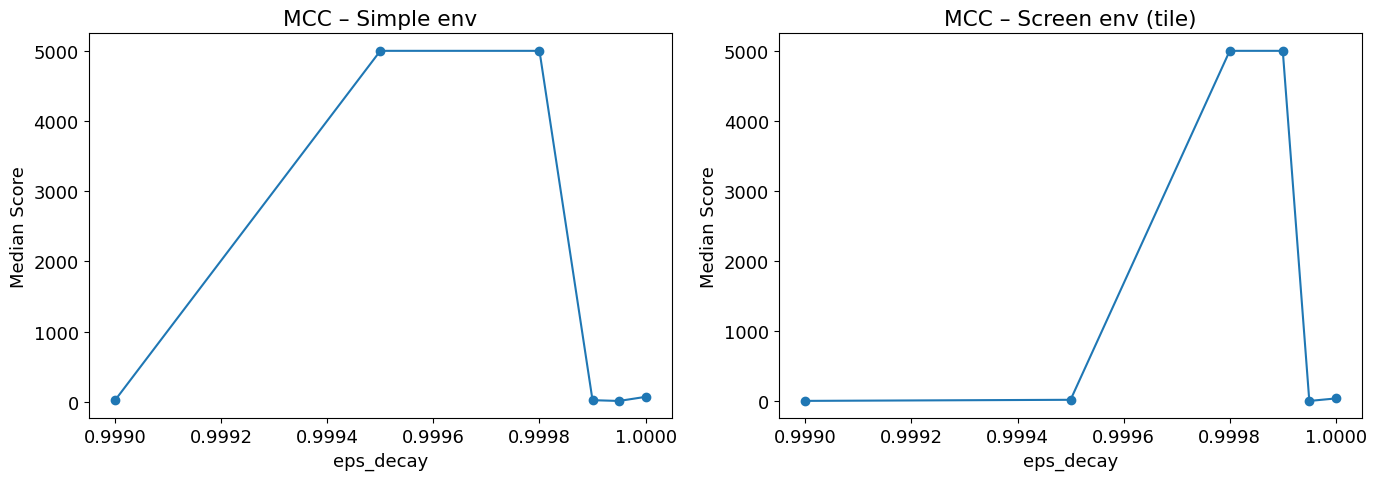
\includegraphics[width=\textwidth]{figures/MCC_eps_decay.png}
    \caption{MCC - Exploration Decay $\epsilon$}
\end{subfigure} 
\hfill
\begin{subfigure}[b]{0.49\textwidth}
    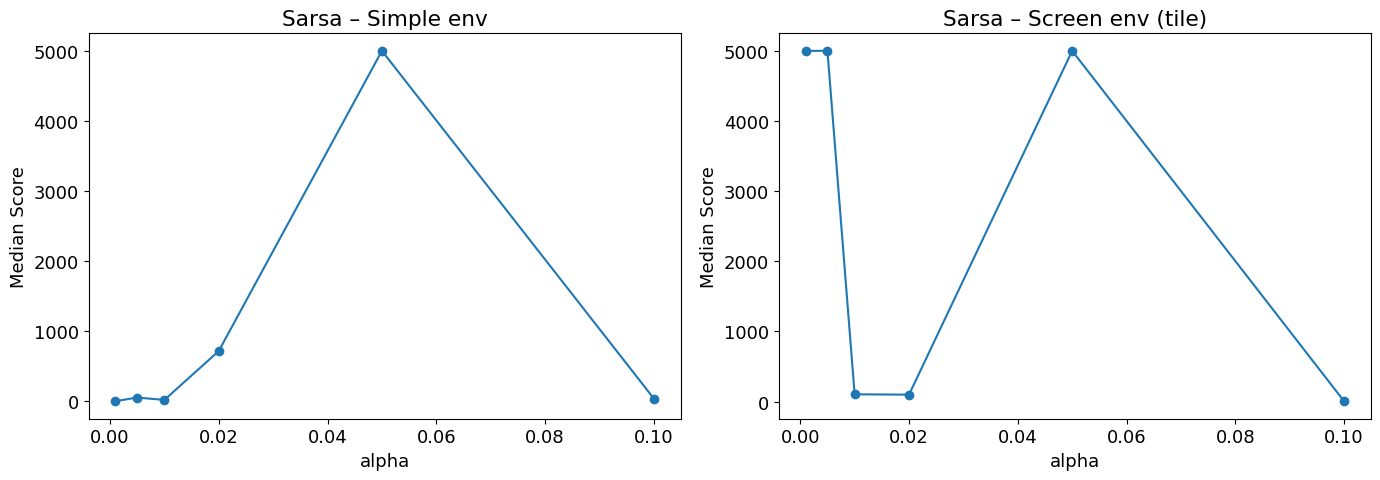
\includegraphics[width=\textwidth]{figures/Sarsa_alpha.png}
    \caption{Sarsa - Learning Rate $\alpha$}
\end{subfigure}
\hfill
\begin{subfigure}[b]{0.49\textwidth}
    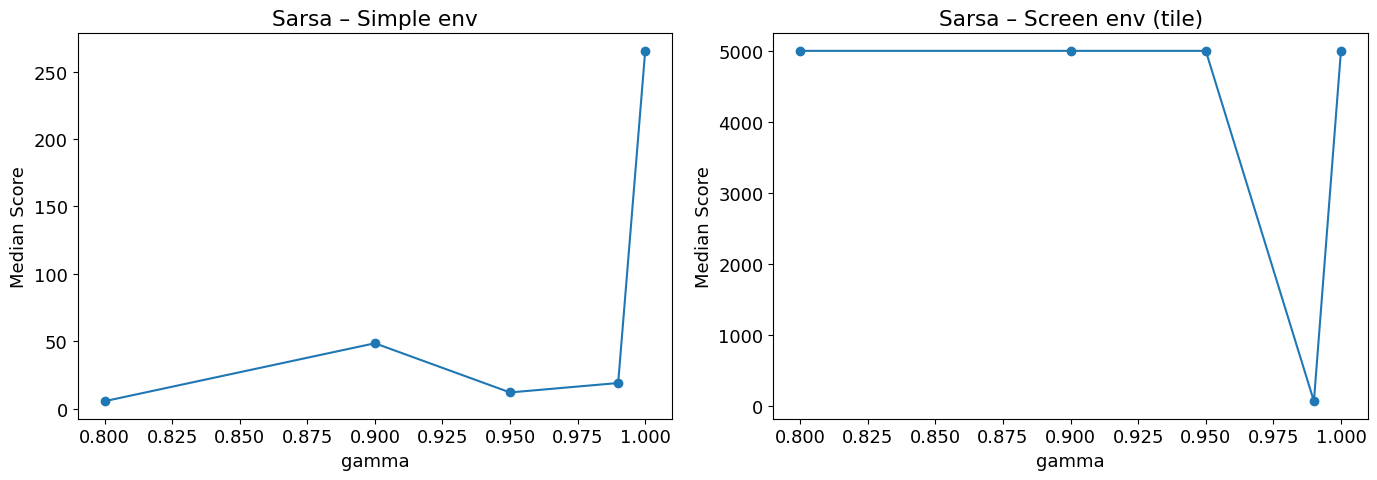
\includegraphics[width=\textwidth]{figures/Sarsa_gamma.png}
    \caption{Sarsa - Discount Factor $\gamma$}
\end{subfigure}
\hfill
\begin{subfigure}[b]{0.49\textwidth}
    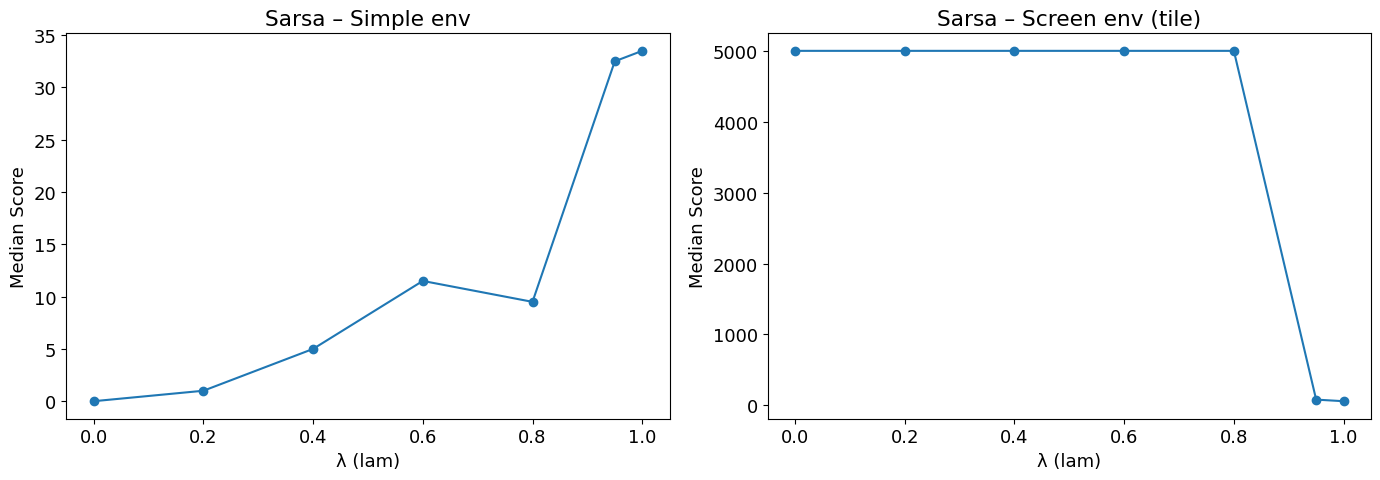
\includegraphics[width=\textwidth]{figures/Sarsa_lambda.png}
    \caption{Sarsa - Trace Decay $\lambda$}
\end{subfigure}
\hfill
\begin{subfigure}[b]{0.49\textwidth}
    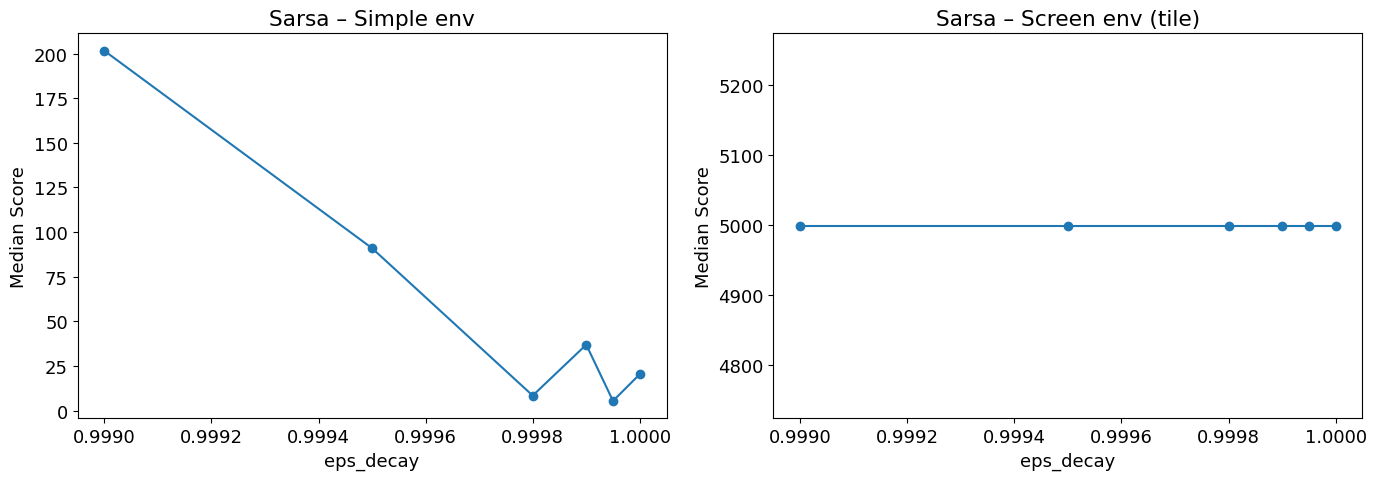
\includegraphics[width=\textwidth]{figures/Sarsa_eps_decay.png}
    \caption{Sarsa - Exploration Decay $\epsilon$}
\end{subfigure}
\caption{Sensitivity analysis of key hyperparameters for the MCC and Sarsa agents. Each plot shows the evaluation performance (score) as a function of the hyperparameter being varied, while keeping the other hyperparameters fixed at their original values. The base configuration used is: $\alpha=0.01$, $\gamma=0.99$, $\lambda=0.8$ (for Sarsa), and $\epsilon$-decay$=0.9998$.}
\label{fig:sensitivity} 
\end{figure}


\end{document}
